%----------------------------------------------------------------------------------------
%	PACKAGES AND THEMES
%----------------------------------------------------------------------------------------
\documentclass[aspectratio=169,xcolor=dvipsnames]{beamer}
\usetheme{SimplePlus}

\usepackage{hyperref}
\usepackage{graphicx} % Allows including images
\usepackage{booktabs} % Allows the use of \toprule, \midrule and \bottomrule in tables

\graphicspath{{./images/}}

%----------------------------------------------------------------------------------------
%	TITLE PAGE
%----------------------------------------------------------------------------------------

\title[short title]{Fair Division} % The short title appears at the bottom of every slide, the full title is only on the title page
\subtitle{Cake Cutting Algorithms: Be Fair if You Can}

\author[Iniyan Joseph] {Iniyan Joseph}

\institute[UTD] % Your institution as it will appear on the bottom of every slide, may be shorthand to save space
{
    University of Texas at Dallas % Your institution for the title page
}
\date{} % Date, can be changed to a custom date


%----------------------------------------------------------------------------------------
%	PRESENTATION SLIDES
%----------------------------------------------------------------------------------------

\begin{document}
% \beamerdefaultoverlayspecification{<+->}

\begin{frame}
    % Print the title page as the first slide
    \titlepage
\end{frame}

\begin{frame}{Overview}
    % Throughout your presentation, if you choose to use \section{} and \subsection{} commands, these will automatically be printed on this slide as an overview of your presentation
    \tableofcontents
\end{frame}

%------------------------------------------------
\section{Introduction to Fair Division}
%------------------------------------------------

\begin{frame}{Introduction}
	Imagine two people want to share this cake.
	\begin{figure}
		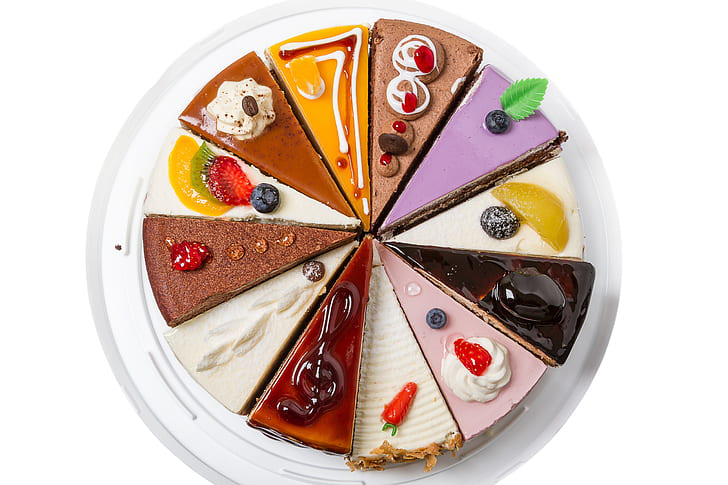
\includegraphics[width=0.75\linewidth]{cakeImage}
	\end{figure}
\end{frame}

%------------------------------------------------
\begin{frame}{Introduction}
    \begin{itemize}
        \item The cake is complicated
        \item The two people may value different parts of the cake differently\pause
        \item Can we come up with an algorithm where both people are happy?
    \end{itemize}
\end{frame}
%------------------------------------------------
\section{Cut and Choose}
%------------------------------------------------
\begin{frame}
	\Huge{\centerline{\textbf{Cut and Choose}}}
\end{frame}
%------------------------------------------------
\begin{frame}{Algorithm}
	\begin{enumerate}
		\item Player 1 cuts the cake into what they believe is half
		\item Player 2 chooses the piece which they think is better
	\end{enumerate}
\end{frame}
%------------------------------------------------
\begin{frame}{Proof of Correctness}
	\begin{enumerate}
		\item Player 1 recieves $\frac{1}{2}$ of the cake
		\item Player 1 values Player 2's allocation to also be worth $\frac{1}{2}$\pause
		\item Player 2 recieved the piece which they thought was better
		\item Player 2 must value their piece to be at least $\frac{1}{2}$ of the cake
	\end{enumerate}
\end{frame}
%------------------------------------------------
\section{Fair Division for $n$}
%------------------------------------------------
\subsection{Banach-Knaster Last Diminisher}
%------------------------------------------------
\begin{frame}
	\Huge{\centerline{\textbf{Banach-Knaster Last Diminisher}}}
\end{frame}
%------------------------------------------------
\begin{frame}{Multiple Columns}
	\begin{columns}[c] % The "c" option specifies centered vertical alignment while the "t" option is used for top vertical alignment
		
		\column{.45\textwidth} % Left column and width
		\textbf{Heading}
		\begin{enumerate}
			\item Statement
			\item Explanation
			\item Example
		\end{enumerate}
		
		\column{.5\textwidth} % Right column and width
		Lorem ipsum dolor sit amet, consectetur adipiscing elit. Integer lectus nisl, ultricies in feugiat rutrum, porttitor sit amet augue. Aliquam ut tortor mauris. Sed volutpat ante purus, quis accumsan dolor.
		
	\end{columns}
\end{frame}
%------------------------------------------------
\begin{frame}{Meeting 2}
	\begin{block}{Agenda}
		\begin{itemize}
			\item Stromquist Envy-Free Moving Knife for n=3
			\item Austin's Perfect Division for n=2
			\item Ideation
		\end{itemize}
	\end{block}
\end{frame}
%------------------------------------------------
%----------------------------------------------------------------------------------------

\end{document}
